\section{Experimento}

\begin{frame}
  \frametitle{Amostragem}
  Pontos de amostragem em Nima.
  \begin{figure}[H]
    \centering
    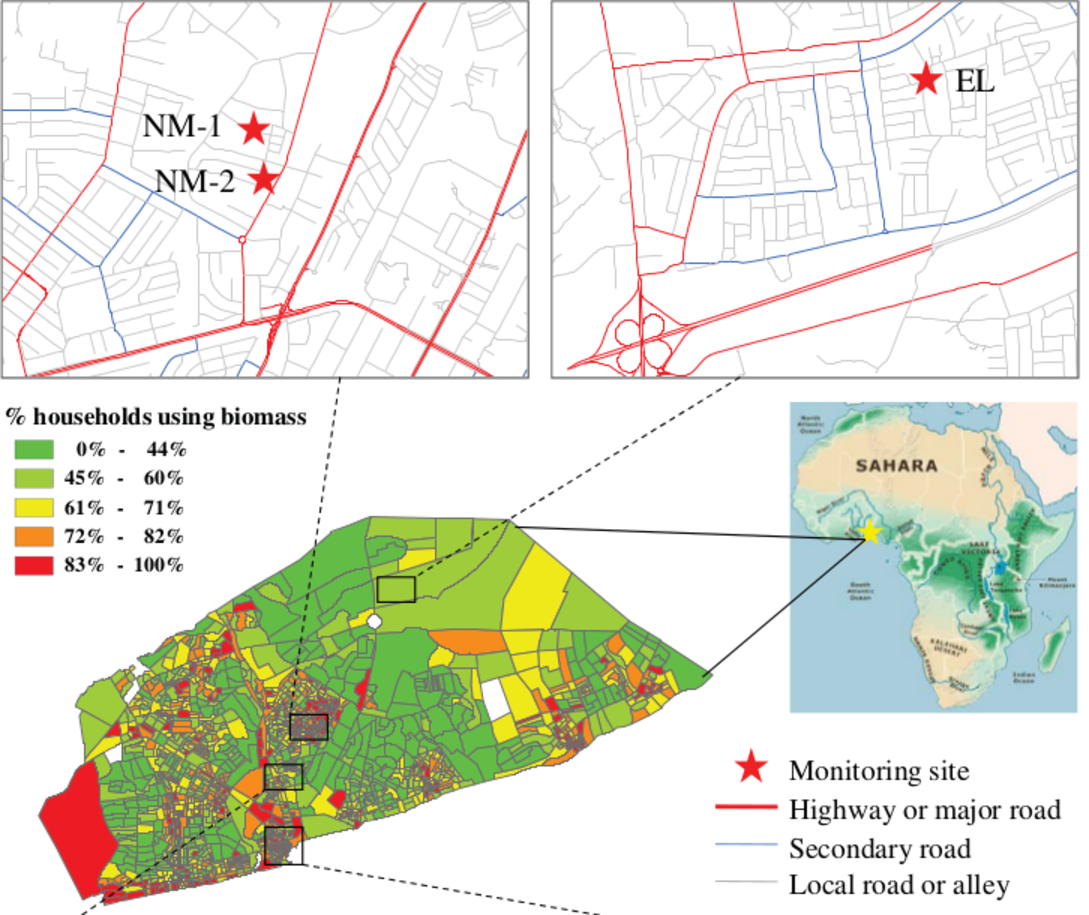
\includegraphics[scale=0.35]{../../../inputs/images/zheng/nima_mapa.pdf}
  \end{figure}
\end{frame}

\begin{frame}
  \frametitle{Meteorologia}
  Distribuição das frequências de direção dos ventos, dados da NOAA.
  \begin{figure}[H]
    \centering
      \includegraphics[scale=0.3]{../../../outputs/ventos_dir.pdf}
      \includegraphics[scale=0.3]{../../../outputs/harmattan2007_2008.pdf}
      
\includegraphics[width=1cm]{../../../inputs/images/rosa_ventos}
  \end{figure}
\end{frame}

\begin{frame}
  \frametitle{Análises}
  \begin{itemize}
    \item Gravimétrica (determinação da massa);  
    \item Refletância (determinação do Black Carbon);
    \item Fluorescência de Raios X (determinação da composição química inorgânica);
  \end{itemize}
\end{frame}

\begin{frame}
  \frametitle{Fluorescência de Raios X - \textit{ED-XRF}}
  Modelamento matemático usado na \textit{ED-XRF}:
  \begin{equation}
	  N_{ij} \propto \frac{m_{ij}}{A_i}I_i{\Delta}t_{i}
  \end{equation}
  Onde,  
  \begin{itemize}
    \item $N_{ij}$ = Contagem de fótons na amostra i para o elemento químico j;
    \item $I_{i}$ = Corrente (ampère) na amostra i;
    \item $\Delta t_i$ = Tempo vivo (segundos) que a amostra i foi irradiada;
    \item \textcolor{red}{$m_{ij}$} = Massa (grama) na amostra i para o elemento químico j;
    \item $A_i$ = Área ($cm^2$)irradiada da amostra i.
  \end{itemize}
\end{frame}

\begin{frame}
  \frametitle{Calibração: Ajuste do Fator de Resposta}
  Constante de proporcionalidade: Fator de Resposta:
  \begin{equation}
    R_j = \frac{A_i}{m_{ij}} \frac{N_{ij}}{I_i \Delta t_i}
  \end{equation}
  \begin{figure}[H]
  \centering
    \begin{minipage}[b]{0.40\linewidth}
      \includegraphics[scale=0.25]{../../../outputs/K2014abril}
    \end{minipage}
    \quad
    \begin{minipage}[b]{0.40\linewidth}
      \includegraphics[scale=0.25]{../../../outputs/L2014abril.png}
    \end{minipage}
  \end{figure}
\end{frame}

\begin{frame}
  \frametitle{Erro no Ajuste - Abordagem matricial mínimos quadrados}
   \begin{equation}
     [R] = A[Z]
   \end{equation}
   
   Sendo $\alpha$ o A ajustado, a covariância dos coeficientes $V_{\alpha}$:
   \begin{equation}
     V_{\alpha} = (Z^t V_R^{-1} Z)^{-1}
   \end{equation}

   O ajuste de A fica:
   \begin{equation}
     \alpha = V_{\alpha} Z^t V_R^{-1} R
   \end{equation}

    Calculando-se os novos valores de R a partir de $V_{\alpha}$:
   \begin{equation}
     [R_{adjusted}] = \alpha[Z]
   \end{equation} 

    A incerteza do ajuste é a raiz quadrada da diagonal da matriz de covariância de $R_{adjusted}$:
   \begin{equation}
     COV_{R_{adjusted}} = Z V_{\alpha} Z^t
   \end{equation} 
\end{frame}

\begin{frame}
  \frametitle{Comparação das análises com a da \textbf{EPA}}
  \begin{figure}[H]
   \centering
    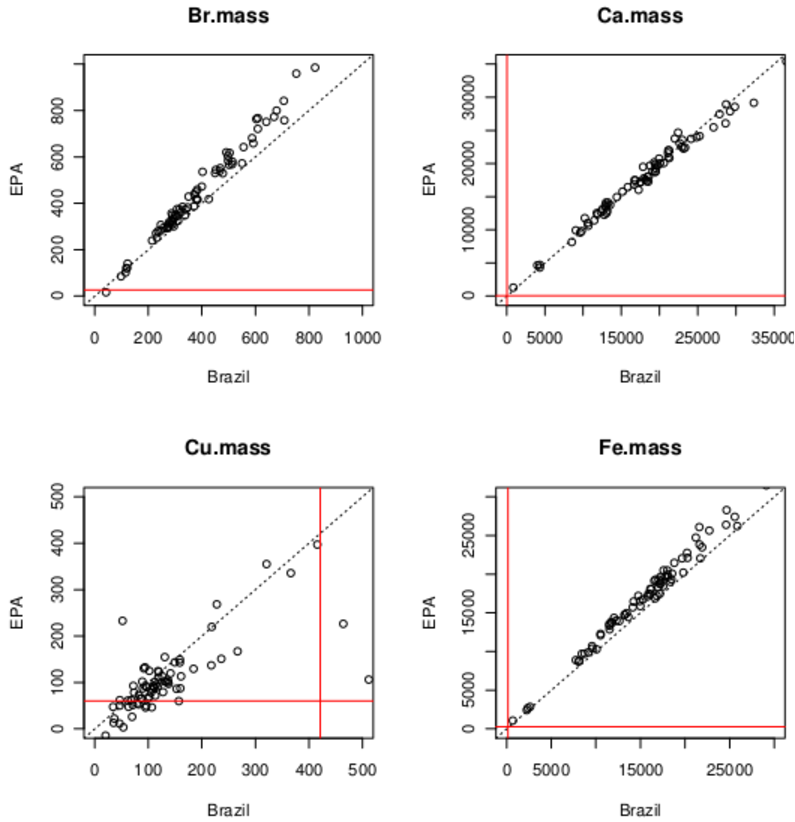
\includegraphics[scale=0.42]{../../../inputs/images/zheng/epa_short_example.PDF}
  \end{figure}
  \begin{tiny}
    2900 amostras - \textbf{USP}. 
    95 de controle pela \textbf{EPA} (US Environmental Protection Agency).
  \end{tiny}
\end{frame}
